\documentclass{sig-alternate}
\usepackage{color}


\newcommand\todo[1]{\textcolor{red}{(#1)}}

\begin{document}

\title{An Overview of Elastic Cloud Applications}
\subtitle{Technical University of Vienna,\\Advanced Internet Computing Lecture,\\
(Jan 2014)}


\numberofauthors{4}
\author{
\alignauthor
Soodeh Farokhi\titlenote{In alphabetical order}\\ %or put the group leader first, if you wish
       1228800
\alignauthor
Gajo Gajic\\
       0828150
\and
\alignauthor
Martin Kalany\\
       0825673
\alignauthor
Jia Wei\\
       0035204
}
       
\date{\today}

\maketitle
\begin{abstract}
\end{abstract}
Cloud computing provides access to a virtually unlimited amount of resources.  In order to realize this feature the cloud provider should be able to support the elastic deployment of applications. Elasticity, the ability to rapidly scale resources up and down on demand, is one of the main advantages of the cloud paradigm and makes it different to an ``advanced outsourcing'' solution.
However, there are various challenges to understand the elasticity requirements of a given application and  several approaches try to tackle these issues. In this paper, we investigate the state of the art of elastic cloud applications and describe the requirements for supporting elasticity in a cloud environment. 
It is because the authors had a working experiment with CloudScale \cite{leitner2012cloudscale}, \cite{Leitner2013} in order to compare the process of deployment an application, twitter-based sentiment analysis, on top of an IaaS (Amazon EC2\footnote{http://aws.amazon.com/ec2/}) by using CloudScale and without using it directly on a PaaS (Google AppEngine \footnote{https://developers.google.com/appengine/}).

\section{Introduction}
More and more enterprises decide to migrate business applications to a cloud environment to utilize the core features of cloud computing, which are, among others: The ability to dynamically increase or decrease computing power on demand as well as a more flexible pay-by-usage model that helps reducing costs associated with running and maintaining a private data/server center. Those costs are significant especially if e.g., high availability and short response times are a requirement. Public cloud providers face serious challenges in order to understand the elasticity characteristics of applications and workloads while having to consider the required capacity of their cloud platforms. 

Ideally, a cloud platform is infinitely and instantaneously elastic, meaning that infinite computing resources are available and that the scaling up of an application can be done instantaneously. Based on this assumption, an application can be scaled out indefinitely with increasing load without increasing response times \cite{brebner2012your}. 

However, supporting this scenario, is not easy to be tackled by Cloud IaaS or PaaS provider. In this paper, we introduce the existing approaches for this problem by considering CloudScale \cite{leitner2012cloudscale} features, advantages and disadvantages over other works as a focus of this work. We will also talk briefly about an experimental comparison between the deployment of a twitter-based sentiment analysis application on Amazon EC2 as a public Cloud IaaS by CloudScale with the deployment of it on Google AppEngine as a public Cloud PaaS without utilizing the CloudScale features as a middleware. It is worth mentioning that, although elasticity is interpreted as the capability of both scaling up and down, while scalability more is used for scaling up, in this paper we used them interchangeable,.

The rest of paper is organized as follows. Section \ref{elasticity-req} discusses the possible ways to provide elastic applications on Cloud and the essential features to support it is explained. Then in Section \ref{sec:rw}, which is the main focus of the paper, the state of the art of elastic cloud applications will be presented in two categories, research work and commercial tools and technologies. In Section \ref{cloudScale} the differences between CloudScale, as a tool which authors had experienced with, and other similar approaches is introduced briefly. Finally, Section \ref{conclusion} concludes the paper.

\section{Elasticity Requirements} \label{elasticity-req}
In general, IaaS or PaaS automatic elasticity in a cloud environment is typically achieved by using a set of provider-defined rules that govern how and when the service should scale up or down to adapt to a varying application load \cite{vaquero2011dynamically}. These rules are a set of conditions that when met trigger some actions on the infrastructure or platform in order to support dynamic scaling. Existing approaches differ greatly in the abstraction level of this process, the customization of rules and the degree of automation.

While some approaches allow the user to specify only simple conditions by using fixed predefined set of metrics such as CPU and memory usage, other approaches offers service level metrics (e.g., cost-to-benefit ratio) in order to allow the user to specify more complex conditions that may further be combinations of simple rules. Existing approaches furthermore differ in the way they behave when the supported conditions are met. Figure \ref{fig:scalabilitymechanisms} ~\cite{vaquero2011dynamically} depicts possible mechanisms of elasticity support on the level of cloud IaaS or PaaS.

Scaling can roughly bew divided in two approaches, called horizontal and vertical scaling. Horizontal scaling is done by either adding new server replicas and load balancers to distribute the load among more servers, or through \todo{what does the following mean? Network scaling is no where defined.} dynamic bandwidth allocation by supporting network scaling. Vertical scaling can be achieved by changing the instances on-the-fly\footnote{without rebooting the machine} either by resizing (e.g. dedicating more physical resources such as CPU and memory to a running virtual machine) or replacing \todo{what?}. However, on-the-fly changes of resources dedicated to a virtual machine instance are not supported by the most common operating systems. Some work like \cite{rodero2010infrastructure} tried to facilitate this process by proposing a new abstraction layer closer to the lifecycle of services, which allows for their automatic deployment and escalation \todo{what?}depending on the service status (not only on the infrastructure). Their proposed abstraction layer sits on top of different cloud providers, hence mitigating a potential lock-in and allowing for a transparent federation of clouds.

Apart from server scalability, load balancing is another major issue for scalability. A load balancer is required to distribute load as evenly as possible among servers or VMs. As a commercial public Cloud IaaS provider, Amazon already has some strategies for load balancing for replicated VMs via the Elastic Load Balancing capabilities \footnote{http://aws.amazon.com/autoscaling/}. Therefore, having several servers and the mechanisms to distribute load among them is a necessary step towards scaling a cloud application \cite{rodero2010infrastructure}. 

However, network scalability \todo{according to  Fig.~\ref{fig:scalabilitymechanisms}, this is only an issue for IaaS} is a somewhat neglected element that should also be considered \cite{wu2009unified} for cloud datacenters in order to be able to support application elasticity. Because several VMs share the same network, potentially producing a huge increase in the required bandwidth, the network too has to be scalable. Regarding to Figure \ref{fig:scalabilitymechanisms}, the aforementioned CloudScale middleware as well as Aneka\footnote{http://www.manjrasoft.com/products.html} and AppScale\footnote{http://www.appscale.com}, which we will introduce in Section \ref{sec:tools}, fall into the "container replication" category \todo{what is this?} in the platform layer (the container is CloudScale here) \todo{how is cloudscale connected to the Aneka and AppScale?}.

\begin{figure*}
\centering
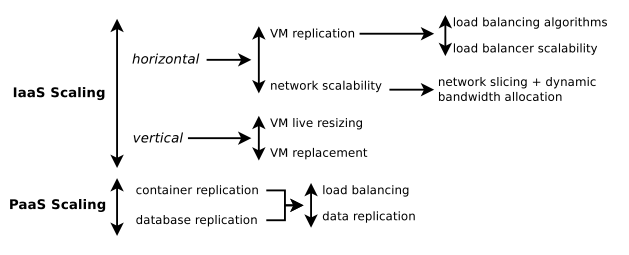
\epsfig{file=figures/ScalabilityMechanisms.png, , width = 10.5cm}
\caption{Possible mechanisms to support elasticity on Cloud IaaS/PaaS ~\cite{vaquero2011dynamically}}
\label{fig:scalabilitymechanisms}
\end{figure*}

\section{Related work}
\label{sec:rw}
In the following, we provide an overview of significant work dealing with elastic cloud applications, where both scientific research and commercial products, technologies and tools are covered.

\subsection{Scientific research}
\label{sec:scientific}
Authors of \cite{keller2013topology} proposes a framework contributes by describing neces-
sary interfaces, functionalities, and data exchanges to deploy complex application across several Cloud IaaS, such as Amazon EC2 in a dynamic and adaptive way. In the other world, they answer the question of "How to deploy elastic applications?" by presenting a flexible framework that supports high-level interfaces for an adaptation plug-in. These interfaces simplify the retrieval of necessary input data for all placement algorithms support state-full applications, or complex application architectures.

In \cite{di2012towards} Aeolus component model is proposed to capture similar scenario from realistic cloud deployments, and specifies compositions of services to automate deployments, planning of day-to-day activities such as software upgrade planning, service deployment, and elastic scaling.

Work presented in \cite{brebner2012your} introduces an elasticity mechanisms of a typical Cloud IaaS platform (inspired by Amazon EC2) and presents a Service Oriented Performance Modeling method and tool to model and predict the elasticity characteristics of three realistic applications and workloads on this cloud platform. They compare the pay-as-you-go instance costs and end-user response time for these three elasticity scenarios. Their proposed model is able to predict the elasticity requirements (in terms of the maximum instance spin-up time) for the working scenarios.

The OSGi-inspired component framework COSCA presented in \cite {kachele2013component} auto- matically manages elastic deployment of component-based application by isolating components of different applications and hides distribution using a virtualized and distributed OSGi-like framework. It eases the usage of cloud resources and scalability for component-based applications. 

The authors of \cite{han2012lightweight} adopts a lightweight approach along with its algorithm to enable cost-effective elasticity for cloud applications. The proposed approach operates fine-grained scaling at the resource level (CPUs, memory, I/O) in addition to VM-level scaling to efficiently scale cloud application’s resources up and down in order to meet the given QoS requirements while reducing cloud providers’ costs.

%--------------------------------------------------------

\subsection{Commercial approaches, technologies and tools}
\label{sec:tools}
Several application provisioning solutions exist, enabling developers and administrators to declaratively specify deployment requirements and dependencies to support repeatable and managed resource provisioning such as Opscode Chef \footnote{www.opscode.com/chef/}, Puppet\footnote{http://puppetlabs.com} and juju\footnote{http://juju.ubuntu.com}. In juju basic services are described as predefined charms and it can fall into the category in which it supports elastic applications by providing help, hints, or triggers.
 
Aneka \cite{vecchiola2009aneka} is a .NET-based platform that focuses on enabling hybrid cloud applications by employing a specialized programming model. It is able to deploy containers and run users applications in several IaaS providers. Aneka is more similar to Grid computing middleware, provides a relatively low-level abstraction based on the message passing interface (MPI). In general, Aneka seems more suitable for building scientific computing applications instead of enterprise applications. 

AppScale \cite{chohan2009appscale} is an open source extension to the Google Ap-
p Engine (GAE) PaaS that allows users to build their own GAE compliant PaaS on top of any private or public IaaS service. Indeed, it provides a framework to investigate the interaction between PaaS and IaaS systems. In order to support the elasticity, it scales the VMs used to host containers depending on actual application demand, automatically configuring the load balancers. It targets Online Transaction Processing (OLTP) style enterprise applications.

Carina Environment Manager\footnote{https://github.com/blackberry/OpenNebula-Carina} automates and speeds up the deployment of services onto the OpenNebula IaaS platform. It supports the automated creation and run-time scaling of multi-VM application environments according to policies. It leverages the OpenNebula contextualization framework to setup clusters of VMs in a master-slave configuration or a set of workers with an IP load-balancer in front. Policies can be defined to control how VMs are added or removed based on manual, time of day, or application load-based triggers.

3Teras AppLogic\footnote{http://www.ca.com/us/cloud-platform.aspx} in another commercial tools to automate complex application deployment. It scales applications without changing code and architecture. Indeed, it provides an on demand scaling by assigning resources to the service as a single entity, rather than a collection of components.

Orleans, introduced in \cite{larus2013look} and \cite{bykov2011orleans} is a software framework developed at Microsoft Research to build reliable, scalable, and elastic cloud applications. It includes programming model that encourages the use of simple, easy to understand and employ concurrency patterns. 
It is based on distributed actor-like components called grains, which are isolated units of state and computation that communicate through asynchronous messages. Orleans enables a developer to concentrate on application logic, while the Orleans runtime provides scalability, availability, and reliability.

CloudBees RUN@Cloud\footnote{http://www.cloudbees.com/} is a service which provides continuous integration and an elastic platform for hosting Enterprise Java Beans (EJB) applications.

%-----------------------------------------------------------------------------------
\section{CloudScale Features} {\label{cloudScale}
In this section, very briefly, we enumerate the features of CloudScale and compare it with the previous introduced approaches in Section \ref{sec:rw}.

CloudScale is a middleware to build applications on top of Cloud IaaS. It provides an abstraction that makes elastic applications running on top of an IaaS seem like regular, non-distributed Java applications. Indeed, it places a middle layer between IaaS offerings, which provide great control over the application, but do so at the costs of high deployment effort, and PaaS offerings, which are easy to use, but provide little control \cite{leitner2012cloudscale}. It allows application developers to have full control over their application, while by using a PaaS, they cannot retain it. Another advantages of using CloudScale is providing an abstract layer by which applications are not bound to any specific cloud providers, and are easy to migrate, work well in the context of private or hybrid clouds, and support a wider variety of applications, while still providing an abstraction comparable to commercial PaaS solutions. CloudScale has a more general claim in comparision with similar approached for elastic applications, which is able to handle a wide variety of elastic application types, including data-intense, processing-intense and OLTP\footnote{Online Transaction Processing} style web applications\cite{Leitner2013}.

Based on \cite{leitner2012cloudscale} the main difference between CloudScale and the introduced approached in Section \ref{sec:rw} are by using CloudScale, developers retain full control over their application. Although CoudScale hides some scalability-related issues from developers, they are still free to customize the way CloudScale works to their own needs, either by implementing customscaling policies, adapting the CloudScale framework itself, or managing some so called Cloud-Objects (regular program-level objects that are abstractions of application logics, and should be distributed over a cloud) in the application manually. The main disadvantage of all of those approaches is that they imply a significant loss of control for the developer and also they typically require the usage of a given public cloud (typically provided by the same vendor), imply the usage of proprietary APIs, and restrict the types of applications that are supported \cite{Leitner2013}.

\section{Conclusion} {\label{conclusion}
In this paper we present the state of the art in elastic Cloud application which include both existing research work and technologies. We also took a look at requirements of supporting elasticity on Cloud. As the authors had experienced with deploying twitter-based sentiment analysis application on IaaS by interfering of CloudScale and without it directly on Google AppEngine, advantages of using CloudScale over existing approaches were discussed briefly as well.

%bibliography ----------------------------------------------------------------------
\bibliographystyle{abbrv}
\bibliography{sigproc} 
\end{document}
